% !TeX program = xelatex
% Authoritative manuscript. Edit this file directly; no document converter is needed.
\documentclass[a4paper,11pt,fontset=none]{ctexart}
\usepackage[margin=2.2cm]{geometry}
\usepackage{fontspec}
\IfFontExistsTF{Times New Roman}{\setmainfont{Times New Roman}}{\setmainfont{texgyretermes-regular.otf}[BoldFont=texgyretermes-bold.otf,ItalicFont=texgyretermes-italic.otf,BoldItalicFont=texgyretermes-bolditalic.otf]}
\IfFontExistsTF{SimSun}{\setCJKmainfont[AutoFakeBold=2]{SimSun}\setCJKmonofont{SimSun}}{\setCJKmainfont[BoldFont=FandolSong-Bold.otf]{FandolSong-Regular.otf}\setCJKmonofont{FandolSong-Regular.otf}}
\usepackage{amsmath,amssymb}
\usepackage{unicode-math}
\setmathfont{latinmodern-math.otf}
\usepackage{graphicx,booktabs,tabularx,array,caption,setspace,microtype,xurl}
\usepackage{placeins}
\usepackage[numbers,sort&compress]{natbib}
\usepackage[hidelinks,unicode]{hyperref}
\hypersetup{pdftitle={非平稳音乐游戏活动排名终分预测的时间一致评测与结构化在线误差校正},pdfauthor={Tano},pdfsubject={时间一致评测与结构化在线误差校正的回溯性研究}}
\urlstyle{same}
\usepackage{fancyhdr}
\newcolumntype{L}{>{\raggedright\arraybackslash}X}
\newcolumntype{C}[1]{>{\centering\arraybackslash}p{#1}}
\captionsetup{font=small,labelfont=bf,justification=justified,singlelinecheck=false}
\renewcommand{\figurename}{图}
\renewcommand{\tablename}{表}
\renewcommand{\refname}{参考文献}
\ctexset{section={format=\large\bfseries\raggedright},subsection={format=\normalsize\bfseries\raggedright}}
\setstretch{1.2}
\setlength{\parindent}{2em}
\setlength{\parskip}{0.25em}
\setlength{\emergencystretch}{3em}
\setlength{\textfloatsep}{12pt plus 2pt minus 2pt}
\setlength{\intextsep}{12pt plus 2pt minus 2pt}
\renewcommand{\topfraction}{0.92}
\renewcommand{\bottomfraction}{0.9}
\renewcommand{\textfraction}{0.05}
\renewcommand{\floatpagefraction}{0.85}
\setcounter{topnumber}{3}
\setcounter{totalnumber}{4}
\pagestyle{fancy}\fancyhf{}\fancyfoot[C]{\small\thepage}
\renewcommand{\headrulewidth}{0pt}
\title{非平稳音乐游戏活动排名终分预测\\的时间一致评测与结构化在线误差校正}
\author{Tano}\date{}
\makeatletter
\renewcommand{\maketitle}{\begin{center}{\fontsize{16}{22}\selectfont\bfseries\@title\par}\vspace{0.6em}{\normalsize\@author\par}\end{center}\vspace{0.5em}}
\makeatother
\begin{document}
\maketitle

\section*{摘要}

\textbf{目的} 音乐游戏限时活动的排名终分预测同时受到活动进度、排名区间、活动规则和历史分布变化的影响。若将同一活动的不同快照随机划分，或在早期预测中混入活动结束后的信息，所得精度难以代表实际应用。\textbf{方法} 以 BanG Dream 国服活动排名汇总分数为研究对象，建立按活动分组且按实际开始时间排序的固定留出、时间网格和逐活动滚动三类评测协议。正文研究队列统一限定于2024年1月29日起的密集采样时期，包含97期活动，按67期训练、14期验证和16期测试划分，覆盖19条排名线。基础预测采用排名共享与上下文增强的梯度提升树；在此前已结束活动的封存预测上计算活动等权对数误差，研究独立指数加权校正、锚点与线间差异分解，以及共享编码、排名专属头、相关线传播和注意力门控等扩展。\textbf{结果} 在相同19线测试面板的5220个前缀上，未校正基线、独立暖启动校正和历史双线组合的活动等权平均绝对百分比误差分别为7.082\%、6.671\%和6.540\%。双线组合相对独立校正的差值为−0.130个百分点，活动配对95\%区间为{[}−0.255，−0.009{]}，但该方案属于历史探索后选用的生产配方。最新一轮按验证集事前选择仍保留独立校正；四种新增神经结构的测试误差为6.716\%至7.240\%，未形成稳定改进。训练期终分的区间内相关中位数为0.979，而早期原始预测误差仅为0.699，上期到本期的相应相关中位数为0.003。\textbf{结论} 分数水平的高相关不足以直接支持跨线残差传播。对于本研究的小样本活动队列，控制信息时间边界并对结构化误差进行低复杂度更新，比增加网络结构更值得优先研究。由于测试队列曾参与探索、验证集反复使用且元数据为回溯快照，结果属于可复现的回溯性证据，仍需独立新活动的前瞻验证。

\textbf{关键词} 活动终分预测；时间序列评测；概念漂移；在线误差校正；跨排名学习；梯度提升树

\clearpage

\section*{Abstract}

\textbf{Time consistent evaluation and structured online error correction for final score forecasting of music game event rankings}

Forecasting final ranking cutoff scores in limited duration music game events requires consistent treatment of event progress, ranking heterogeneity, and temporal changes. We investigate aggregated ranking scores from the Chinese server of BanG Dream using a frozen dense sampling cohort of 97 events, chronologically divided into 67 training, 14 validation, and 16 test events. Three protocols separate fixed holdout evaluation, a 21 origin temporal grid, and eventwise rolling updates. A gradient boosted backbone is combined with corrections learned exclusively from sealed forecasts of events completed before the current event starts. We compare independent exponentially weighted corrections, an anchor and contrast decomposition for T1000 and T2000, and neural extensions using shared representations, rank specific heads, related rank information, and attention gating. On the identical 19 rank test panel with 5220 prefixes, event macro mean absolute percentage errors are 7.082\% for the uncorrected backbone, 6.671\% for independent warm correction, and 6.540\% for the historically best paired combination. The paired combination improves on independent correction by 0.130 percentage points, with a paired event 95\% interval of {[}−0.255, −0.009{]}. This combination was adopted after historical exploration and is not a newly confirmed validation winner. In the latest prespecified validation comparison, independent correction remains selected; the four additional neural architectures achieve test errors between 6.716\% and 7.240\%. Strong correlations between score levels weaken markedly for remaining growth and forecast errors. These findings favor parsimonious, structurally targeted adaptation over indiscriminate information sharing in this small event cohort. Previously explored test events, repeatedly used validation data, and retrospective metadata limit confirmatory interpretation. Prospective evaluation on newly completed events remains necessary.

\textbf{Keywords} final score forecasting; temporal evaluation; concept drift; online error correction; cross rank learning; gradient boosting

\section{引言}

限时排名活动将玩家行为汇总为随时间变化的竞争分数。对目标排名线而言，活动中途已经观测到的分数并不等于最终进入该排名所需的分数：活动时长、剩余时间、阶段性增长和结束前集中投入共同决定后续增长。以T1000为例，本文的预测对象是活动结束时第1000名对应的汇总分数，而不是某个固定玩家的个人得分。该任务可被视为具有共同活动背景、多个排名层级和延迟终点标签的条件时间序列回归问题。

这类问题的难点不仅在于拟合曲线。第一，同一活动的多个排名和多个时间点共享一个潜在活动环境；把这些快照视为独立样本容易高估有效样本量。第二，活动结束后的终分对于下一期可能是合法历史，却不能进入本期早期预测。固定留出与滚动更新回答不同的问题，二者不应混为同一模型比较。第三，排名线之间的共同热度可能造成很高的分数相关性，但预测目标是尚未发生的剩余增长；高水平相关并不自动意味着残差也适合共享。第四，采样机制发生变化时，早期稀疏曲线可能无法支持与密集曲线相同的局部速率和末期冲刺特征。

在线学习与概念漂移研究讨论了输入与目标关系随时间变化时的适应策略\citep{gama2014drift}。预测评测研究强调滚动预测起点、重估参数与多测试时期的作用\citep{tashman2000evaluation,cerqueira2020evaluation}。在模型层面，梯度提升树能够处理不规则的表格特征关系\citep{prokhorenkova2018catboost,chen2016xgboost}；LSTM、时间卷积网络和基于分块的Transformer则为曲线表征提供了不同的归纳偏置\citep{hochreiter1997lstm,bai2018tcn,nie2023patchtst}。近年来的表格和时间序列基础模型扩展了小样本预测与零样本预测的选择范围\citep{hollmann2025tabpfn,das2024timesfm,ansari2025chronos2}。然而，这些方法在公开基准上的优势不能替代目标应用中对样本相关性、时间边界和匹配基线的检查\citep{grinsztajn2022tabular}。

本文围绕四个研究问题展开：如何使活动终分预测的离线评测与实际信息到达顺序一致；历史误差校正能否在相同基础预测上带来收益；哪些跨线关系可能具有可用的预测意义；以及共享编码、专属输出头和相关线学习能否超越简单校正。本文的工作包括：构建保持活动归属不变的三层评测体系；给出仅从合法历史封存预测构造的锚点与差异校正；报告跨排名关联的分层统计诊断；并在保留负结果的前提下整理静态模型、在线统计方法和神经网络的匹配实验。

本研究定位为单一应用场景的回溯性方法研究，而非已完成外部验证的普适预测算法。历史最佳配方、每轮验证事前选择和最终生产采用是三个不同事实，本文分别报告，不以事后测试排序替代正式选择过程。

\section{数据与时间一致评测}

\subsection{数据来源与预测对象}

数据来源为Bestdori公开的BanG Dream活动、排名分数和活动元数据\citep{bestdori2026data}，研究使用国服实际开始和结束时间。每条曲线由活动、排名和带时间戳的分数序列组成。元数据包括活动类型、角色和乐队组成，以及具有国服发布时间的卡牌条目。统计与建模均使用排名汇总分数，不涉及玩家身份特征。

设活动为 \(e\)，排名为 \(r\)，开始与结束时间分别为 \(S_e\) 和 \(E_e\)。在名义预测时刻 \(t\)，最后一个合法观测的实际时刻为 \(u_{e,r,t}\leq t\)，对应分数为 \(x_{e,r,t}>0\)；目标为结束时的真实分数 \(Y_{e,r}>0\)。有效前缀至少包含4个观测点，且 \(t-u_{e,r,t}\leq60\ \mathrm{min}\)。完整历史曲线至少包含5个点，并要求末次终点观测位于活动结束前1分钟至结束后5分钟的质量窗口。该终点窗口用于核实已结束标签，不允许在早期预测中读取未来点。

研究覆盖T10、T20、T30、T40、T50、T100、T200、T300、T400、T500、T1000、T1500、T2000、T3000、T4000、T5000、T10000、T20000和T30000，共19档。不同档位的覆盖并不完全相同。T1500在冻结训练与验证组均无合格曲线，测试组有14期、242个前缀；T10的验证和测试曲线各为13期。所有方法沿用同一可用案例名单，不因模型误差而删除困难样本。

\subsection{密集采样时期与冻结活动队列}

正式研究数据统一满足 \(S_e\geq1706504400000\ \mathrm{ms}\)，即北京时间2024年1月29日13时。采用实际时间比较，活动ID仅作为标识。采样诊断显示，在原冻结训练集的边界前186期活动中，每条曲线活动内观测点数的中位数为31、典型间隔中位数为165.5分钟；边界后的12期早期密集活动相应为335.5和30.0分钟。该诊断仅用于说明观测机制差异，既不是全部97期的密度估计，也不是正式的采集系统变点检验。将早期稀疏记录排除是数据适用范围的约束，不能把新旧队列总分之差解释为该处理的因果收益。

从原合格活动名单按上述实际开始时间筛选出97期，再按70\%、15\%与余数划为67、14和16期。训练、验证、测试的活动归属在所有协议与排名之间共享。活动ID存在与实际时间不一致的排序，因而不按ID区间重建分组。表~\ref{tab:cohort}给出活动的真实时间范围。

项目早期原版队列包含283期活动，分为198期训练、42期验证和43期测试，使用较早的采样覆盖。该历史队列及其预测保留用于追溯，原始与密集时期的结果分别归档。下文V1、V2和V3均明确指本节定义的密集时期版本，不把删除早期资料前后的总分差作为模型提升证据。

\begin{table}[!htbp]
\centering
\caption{冻结密集采样队列的活动归属}\label{tab:cohort}
\small
\setlength{\tabcolsep}{4pt}
\renewcommand{\arraystretch}{1.18}
\begin{tabular}{l r c c c}
\toprule
分组 & 活动数 & 最早开始日期 & 最晚开始日期 & 最晚结束日期 \\
\midrule
训练 & 67 & 2024-01-29 & 2025-11-30 & 2025-12-09 \\
验证 & 14 & 2025-12-11 & 2026-04-26 & 2026-05-04 \\
测试 & 16 & 2026-05-06 & 2026-10-16 & 2026-10-24 \\
\bottomrule
\end{tabular}
\end{table}

\subsection{固定留出与时间网格协议}

V1保留训练组拟合、验证组选参和测试组独立评分的固定留出法。验证和测试使用25\%、50\%、75\%进度及结束前24小时、6小时五个评测条件；训练前缀沿用冻结训练采样。V2在不改变活动归属的前提下，扩展为三个时间轴的21个名义条件：开始后1、3、6、12、24、48、72小时；10\%、25\%、50\%、75\%、90\%、95\%进度；以及结束前48、24、12、6、3、1、0.5、0.25小时。真实预测时刻及实际观测滞后均保留。同一活动、排名与物理时刻若对应多个条件，只生成一个案例并通过成员关系引用，总体指标不重复计数。

V1与V2的预处理、编码、模型拟合和完整历史统计只能使用训练组。对于训练样本自身的历史特征，还必须排除本期及在其开始时尚未结束的活动。验证与测试终分不回灌模型。卡牌特征按国服发布时间过滤，另一条排名线也只能使用截至本线实际观测时刻的前缀。

\subsection{逐活动滚动协议与延迟反馈}

V3保留V2的案例、时间网格和活动归属，但允许在活动结束后，将其真实结果用于后续活动。对当前活动 \(e\)，合法历史池为
\begin{equation}\label{eq:history}
\mathcal H_e=\{j:S_j\geq S_{\min},\ E_j<S_e\}.
\end{equation}

本期所有排名和时间点共享期初历史池；当前活动进行过程中，基础模型与误差状态固定。每期先生成并封存预测，再由独立协调器在时间守卫允许后释放结果。模型不直接读取隔离答案库。预处理、类别字典及残差状态也必须与该期历史池一致。验证仅选择预先登记的更新规则；进入测试后规则固定，后续终分只触发该规则的正常更新。

图~\ref{fig:protocol}展示本文暖启动扩展使用的32期基础热身与35期训练期因果预测。最初32期仅建立基础模型，其后35期依次预测、封存，再释放终分，形成真实外推误差，而不是训练拟合残差。随后依次处理14期验证与16期测试，共65个发布预测的查询活动。较早的冷启动校正实验将67期全部作为基础训练初始池，校正从验证期开始积累；这种差异以单独匹配控制呈现，不能把额外的残差历史当成更复杂算法的收益。

\begin{figure}[!htbp]
\centering
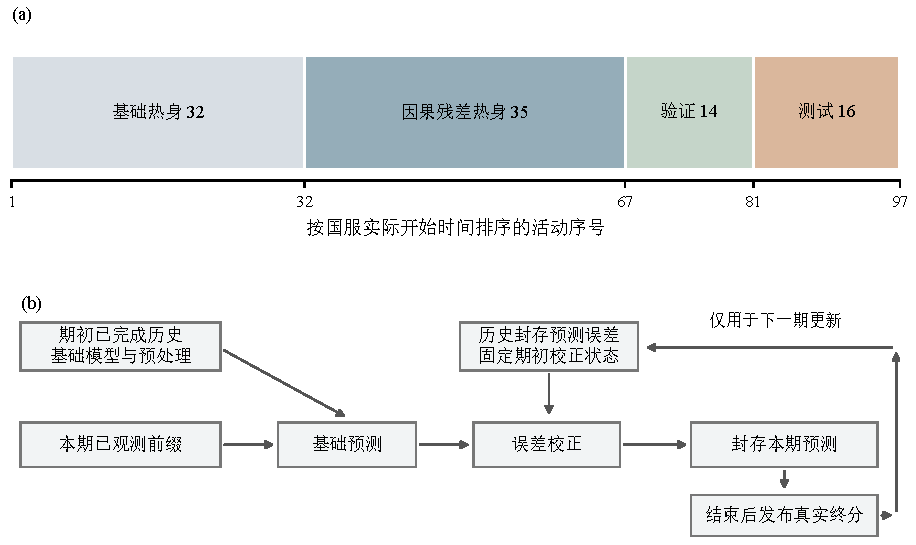
\includegraphics[width=15.8cm,height=\textheight,keepaspectratio]{figures/causal_evaluation_protocol.pdf}
\caption{活动分组与预测先于反馈的时间顺序。上图横轴为按实际开始时间排列的活动顺序，并非等间隔日历时间；下图的本期终分仅用于下一期更新。}
\label{fig:protocol}
\end{figure}

\begin{table}[!htbp]
\centering
\caption{三类协议的有效前缀数量与信息条件}\label{tab:protocols}
\small
\setlength{\tabcolsep}{4pt}
\renewcommand{\arraystretch}{1.18}
\begin{tabularx}{\linewidth}{L r r r L}
\toprule
协议与范围 & 训练前缀 & 验证前缀 & 测试前缀 & 验证与测试终分回灌 \\
\midrule
V1 两线 & 2390 & 130 & 154 & 不允许 \\
V2 两线 & 2452 & 488 & 560 & 不允许 \\
V2 19线 & 21984 & 4361 & 5220 & 不允许 \\
V3 两线 & 2452 & 488 & 560 & 仅已结束活动用于后续活动 \\
V3 19线 & 21984 & 4361 & 5220 & 仅已结束活动用于后续活动 \\
\bottomrule
\end{tabularx}
\par\vspace{4pt}
\begin{minipage}{\linewidth}\footnotesize\setstretch{1.1}
注：V3训练列为父数据集全部可用前缀，不等于校正器的监督样本数。暖启动实验实际使用35期训练活动的1282个两线或11536个19线因果前缀；最初32期不报告外推精度。验证19线面板实际仅覆盖18条有标签线。
\end{minipage}
\end{table}

\section{基础预测与结构化在线误差校正}

\subsection{有界增长解码与基础模型}

定义实际观测进度 \(p_{e,r,t}=(u_{e,r,t}-S_e)/(E_e-S_e)\)。基础模型以经过进度调整的对数增长为监督目标，解码为
\begin{equation}\label{eq:target}
\begin{aligned}
z_{e,r,t}&=\log\frac{Y_{e,r}}{x_{e,r,t}}+\log p_{e,r,t},\\
\widehat Y^{(0)}_{e,r,t}&=x_{e,r,t}\exp\!\left[\operatorname{clip}\{f_{\theta_e}(X_{e,r,t})-\log p_{e,r,t},0,4\}\right].
\end{aligned}
\end{equation}

该设计将简单的``当前分数除以进度''作为增长尺度上的参照，并约束输出位于当前分数与其 \(\exp(4)\) 倍之间。上界属于固定的计算稳定性约束，不是对游戏机制的理论界限。若公开榜单因清除异常记录等原因出现分数下降，下限约束可能成为失配来源；生产训练会单独记录并排除当前分数已超过核实终分的监督前缀，保留原始曲线与真实终分。该生产策略与冻结评测名单分开，不能利用它改善历史测试名单。

T1000与T2000使用上下文增强的400树CatBoost模型，树深4、学习率0.04、叶节点L2系数12、随机种子42。输入涵盖当前分数、实际进度、剩余时间、局部速率、曲线形态，以及合法历史中的活动类型、乐队和角色组成、可用卡牌与历史增长统计。其余17档采用600树共享排名模型，树深5、学习率0.035、叶节点L2系数12，并使用连续对数排名、活动类型、局部统计和33个归一化前缀形态坐标。共享排名配方不等同于两线上下文模型，不将未加入的乐队特征表述为所有排名共有输入。

所有监督拟合按活动等权：若活动 \(e\) 有 \(m_e\) 个训练前缀，则每个前缀的相对权重为 \(1/m_e\)。较高采样密度或较多可用排名不会增加单个活动的总训练权重。缺失值处理与类别编码仅拟合当时合法历史；新类别使用明确的未知处理，不能由当前查询批次反向调整预处理。

\subsection{从封存预测形成活动误差}

令阶段 \(q\) 由实际进度划为 \([0,0.25)\)、\([0.25,0.9)\) 和 \([0.9,1)\)。对已结束活动 \(j\)，先在同一排名、同一阶段的封存基础预测上计算
\begin{equation}\label{eq:error}
\bar\epsilon_{j,r,q}=\frac{1}{|\mathcal C_{j,r,q}|}\sum_{t\in\mathcal C_{j,r,q}}
\log\frac{\widehat Y^{(0)}_{j,r,t}}{Y_{j,r}}.
\end{equation}

正误差表示基础模型偏高，因此后续校正应从预测的对数尺度中扣除。每期每线每阶段只贡献一个均值，不把快照数量转换为更多独立反馈。输入只能来自在发布时已经封存、且当前活动开始前已经结束的查询活动；基础模型在训练集上的拟合误差不能替代式~\eqref{eq:error}。历史记录按结束时间、实际开始时间和活动标识稳定排序。

\subsection{独立指数加权与支持度收缩}

指数加权移动平均以几何衰减方式追踪近期偏差\citep{roberts1959ewma}。对某一排名与阶段的合法历史误差序列 \(a_1,\ldots,a_n\)，定义 \(\operatorname{EWMA}_{\alpha}(a_{1:n})\) 为以首个误差初始化、之后按 \(v_k=(1-\alpha)v_{k-1}+\alpha a_k\) 更新的末值。独立校正为
\begin{equation}\label{eq:independent}
b^{\mathrm{ind}}_{e,r,q}=\operatorname{clip}\!\left\{
\frac{n_{e,r,q}}{n_{e,r,q}+10}
\operatorname{EWMA}_{0.3}(\bar\epsilon_{1:n,r,q}),-0.3,0.3\right\}.
\end{equation}

当历史为空时取零；支持度收缩限制少量活动产生的大幅修正。该规则按活动而非按日历天衰减，因此遇到不同活动间隔时并非固定时间半衰期滤波器。本文将其作为固定的简单参考，而非宣称其对所有排名都最优。

\subsection{T2000锚点与T1000差异分解}

为了使两条线以不同速度适应变化，先用T2000自身的历史阶段误差构造锚点，再对同时具有两线误差的活动构造差值。设锚点支持数为 \(n_a\)，配对支持数为 \(n_d\)，有
\begin{equation}\label{eq:anchor}
\begin{aligned}
A_{e,q}&=\frac{n_a}{n_a+10}\operatorname{EWMA}_{0.2}(\bar\epsilon_{j,2000,q}),\\
D_{e,q}&=\frac{n_d}{n_d+5}\operatorname{EWMA}_{0.6}(\bar\epsilon_{j,1000,q}-\bar\epsilon_{j,2000,q}).
\end{aligned}
\end{equation}
\begin{equation}\label{eq:paired}
\begin{aligned}
b^{\mathrm{pair}}_{e,2000,q}&=\operatorname{clip}(A_{e,q},-0.3,0.3),\\
b^{\mathrm{pair}}_{e,1000,q}&=\operatorname{clip}(A_{e,q}+D_{e,q},-0.3,0.3).
\end{aligned}
\end{equation}

T2000锚点可使用该线全部合法历史，差异项仅使用同一期同时具有两线阶段误差的配对历史，二者支持数不必相同。没有配对历史时，T1000回退至式~\eqref{eq:independent}；T2000没有自身历史时也回退至自身独立状态。所有其他排名继续使用式~\eqref{eq:independent}。最终预测为
\begin{equation}\label{eq:decode}
\widehat Y_{e,r,t}=\operatorname{clip}\!\left\{
\widehat Y^{(0)}_{e,r,t}\exp[-b_{e,r,q(t)}],\ x_{e,r,t},\ x_{e,r,t}\exp(4)\right\}.
\end{equation}

这一分解共享的是历史误差中的锚点与相对差异，不要求两条线的当期真实误差高度相关，也不读取另一条线尚未知晓的终分。它可以由低维递归状态实现，数学上不是通常意义的深层残差网络。本文将其称为``双线组合''，与后续具有可学习参数的残差神经网络分别讨论。

\subsection{神经网络与跨线共享扩展}

研究依次考察条件残差MLP、共同与差异双头网络、活动条件专家门控、多线门控，以及共享编码与排名专属头。静态序列模型包括LSTM、TCN与PatchTST类结构；TabPFNv2通过重新构造训练集上下文预测，不对预训练权重进行任务微调；Chronos-2与TimesFM2.5作为零样本基线。三者的适用输入和推理机制不同，不把零样本推理称为任务重训。

最新一轮四种网络共享同一组基础分数和独立暖校正，在其剩余误差上学习增量：共享编码与共享输出、增加每线专属线性头、增加静态相关线消息、进一步增加阶段图与注意力门控。编码器宽度为16和16，共享输出头宽度为8和1。专属头随本线历史支持度收缩，未见排名不启用本线专属头。关系图仅由当时已经结束活动的历史参考误差构造，每对至少8个活动才使用样本相关，每线最多保留3个邻居；支持不足时采用固定的对数排名距离先验。

四种网络均固定训练60轮，使用AdamW、学习率0.002、权重衰减0.05和0.1丢弃率。训练损失为活动等权百分比误差并带小幅增量惩罚。历史不足12个已发布活动时回退至参考。随机种子固定为42、123和2026，最终模型取三个种子的预测终分算术平均。当前活动的同行前缀裁剪至本线实际观测时刻，超过1小时滞后的同行观测带缺失掩码。当前特征不能拟合标准化，历史前缀保留其原发布时的关系图，不用后来结果改写历史图。

\section{实验设计与统计分析}

\subsection{比较层级与主要终点}

历史研究包含密集时期14个正式运行、329组方法、种子或组合记录；329不是独立网络结构数。本文首先整理V1、V2中的静态结果，说明训练拟合与后续活动外推的差异；随后以相同V3基础预测上的匹配控制作为主要比较。最新19线实验的验证面板为14期、4361个前缀，测试面板为16期、5220个前缀。原两线面板仍为相同16期、560个前缀。

主指标为活动等权MAPE。设测试活动集合为 \(\mathcal E\)，活动 \(e\) 的唯一案例集合为 \(\mathcal C_e\)，定义
\begin{equation}\label{eq:metric}
\operatorname{MAPE}_{\mathrm{event}}=
\frac{100}{|\mathcal E|}\sum_{e\in\mathcal E}
\frac{1}{|\mathcal C_e|}\sum_{i\in\mathcal C_e}
\left|\frac{\widehat Y_i-Y_i}{Y_i}\right|.
\end{equation}

该指标使每个活动的总权重相同，并不额外保证所有排名在缺测条件下完全等权。另报告案例MAPE、MAE、RMSE和案例APE的第90百分位。不同排名量级差异较大，MAE和RMSE可能被高分排名主导；MAPE也并非无偏或对称的预测损失\citep{hyndman2006metrics,demyttenaere2016mape}，因此不能以某个单一指标下降替代全面评价。

验证集只在事前固定菜单内选择方法，测试答案由独立评分器读取。每轮正式主结果与历史描述性控制保持原标记。最终生产组合虽然在已知测试中最好，但不是最新一轮验证选中的方法；本文不重写这一事实。各协议的信息条件或时间点不同，总分分列而不直接相减。

\subsection{匹配比较与不确定性}

对方法A和B，先在相同案例上计算每个活动的MAPE差值，再对完整活动进行5000次配对重采样，随机种子为42。另保留长度为3与5个活动的循环移动块重采样，考察相邻活动相关带来的敏感性\citep{kunsch1989bootstrap}。主文同时展示活动配对与5活动块95\%百分位区间。块长度按活动计数，而非固定日历时长；仅16期测试时，区间依赖的近似平稳条件很弱，应视为面板敏感性描述。

模型比较区间没有对多方法探索和事后关注进行校正，不能据区间不跨零就声称完成了确认性显著性检验。反复优化有限验证集同样可能造成选择偏差\citep{cawley2010selection}。本文保留全部候选、逐种子结果和预先选择记录，不通过删掉较差结构或单独挑选某个种子提高主成绩。

\subsection{跨排名统计诊断}

统计分析区分终分水平、条件调整后的终分、剩余增长、同期预测误差以及跨期误差。主要系数为Spearman相关。终分与剩余增长只使用训练活动；误差使用35期训练组的因果逐期预测，每期每线每阶段先汇总，再计算关联。按预先固定的T10--T50、T100--T500、T1000--T5000和T10000--T30000区间，分别统计区间内与跨区间线对的相关中位数。

偏秩相关通过时间、活动时长的秩与活动类型、乐队哑变量做线性投影，不能视为已控制全部混杂的因果估计。T1500的训练期相关矩阵保持缺失，不填零；补充盲前缀分析可以包含该线，但不把前缀水平相关当作已知终分或增长规律。跨期关系进一步使用循环位移及全局BY校正\citep{benjamini2001by}作探索性筛查，报告小样本检验力限制。

\section{结果}

\subsection{静态模型存在明显的验证与测试落差}

表~\ref{tab:static}给出相同密集时期V2两线面板上的代表性方法。各神经网络主结果采用三种子终分平均，未单独挑选最有利种子。基础树模型训练拟合MAPE为3.611\%，验证为6.430\%，测试为12.755\%；双线TCN训练拟合为3.000\%，验证为5.560\%，测试为14.392\%。更低的训练或验证误差未稳定转化为后续活动测试收益。

\begin{table}[!htbp]
\centering
\caption{V2两线静态模型与基础模型探索}\label{tab:static}
\small
\setlength{\tabcolsep}{4pt}
\renewcommand{\arraystretch}{1.18}
\begin{tabularx}{\linewidth}{L p{3.0cm} C{1.7cm} C{1.7cm} C{1.7cm}}
\toprule
方法 & 训练指标性质 & 训练MAPE / \% & 验证MAPE / \% & 测试MAPE / \% \\
\midrule
排名共享CatBoost & 训练拟合 & 3.611 & 6.430 & 12.755 \\
双线TCN三种子均值 & 训练拟合 & 3.000 & 5.560 & 14.392 \\
阶段路由组合 & 训练拟合 & 2.203 & 4.852 & 13.259 \\
检索残差模型 & 训练拟合 & 3.602 & 5.355 & 23.141 \\
后续模型组合 & 训练拟合 & 2.277 & 4.658 & 14.062 \\
双时钟增长网络 & 训练拟合 & 5.196 & 9.299 & 12.577 \\
进度增长网络 & 训练拟合 & 5.402 & 9.605 & 12.398 \\
多时距进度辅助监督 & 训练拟合 & 5.587 & 9.262 & 12.129 \\
TabPFNv2上下文增强 & 上下文重代入诊断 & 0.931 & 5.979 & 12.747 \\
TabPFNv2基础配方 & 上下文重代入诊断 & 2.246 & 6.598 & 13.074 \\
Chronos-2 & 零样本推理 & — & 33.842 & 31.131 \\
TimesFM2.5 & 零样本推理 & — & 38.057 & 35.125 \\
\bottomrule
\end{tabularx}
\par\vspace{4pt}
\begin{minipage}{\linewidth}\footnotesize\setstretch{1.1}
注：TabPFN的训练查询也在上下文内，训练列不能视为外推精度；零样本模型不报告``训练拟合''。上述方法来自既有不同固定菜单，表格用于描述，不把全表测试最低者重新定义为事前主结果。各配方的输入表达和计算预算并非统一最优调参预算，结果不证明这些通用架构在其他实现或任务中无效。
\end{minipage}
\end{table}

V1五时点的事前主方法为截止时间特征模型，测试MAPE为14.39\%；V2两线跨菜单事前选择为后续模型组合，测试为14.06\%；V2的19线共享树模型测试为7.50\%。这些值对应不同预测时点或排名范围，不构成逐项可相减的模型进步曲线。后文改用同一V3面板上的基础预测与校正器对照，以分辨校正本身的贡献。

\subsection{简单滚动校正与历史双线组合}

表~\ref{tab:main}汇总相同V3的19线面板。未校正基线的验证与测试MAPE为6.672\%和7.082\%；独立暖校正分别为6.502\%和6.671\%，测试相对下降5.80\%。双线组合分别为6.556\%和6.540\%，相对未校正基线下降7.65\%，相对独立暖校正下降1.96\%。最后一个差异为0.130个百分点，而不是下降1.96个百分点。

\begin{table}[!htbp]
\centering
\caption{相同19线V3案例上的主要比较}\label{tab:main}
\small
\setlength{\tabcolsep}{4pt}
\renewcommand{\arraystretch}{1.18}
\begin{tabularx}{\linewidth}{L p{3.1cm} C{1.65cm} C{1.85cm} C{1.85cm}}
\toprule
方法 & 证据角色 & 验证MAPE / \% & 19线测试MAPE / \% & 原两线测试MAPE / \% \\
\midrule
未校正基础预测 & 描述性基线 & 6.672 & 7.082 & 12.008 \\
独立暖校正 & 最新一轮事前选择 & 6.502 & 6.671 & 7.740 \\
历史双线组合 & \shortstack[l]{历史最佳\\生产采用} & 6.556 & 6.540 & 6.540 \\
多线门控网络 & 既有神经控制 & 6.559 & 6.658 & 7.204 \\
相邻排名图校正 $\lambda=1$ & 上一轮事前选择 & 6.435 & 6.938 & 10.399 \\
共享编码与共享输出 & 新增候选 & 6.617 & 6.716 & 7.819 \\
共享编码与每线专属头 & 新增候选 & 6.917 & 7.240 & 9.151 \\
增加静态相关线信息 & 新增候选 & 6.877 & 7.213 & 9.326 \\
增加阶段图与注意力 & 新增候选 & 6.813 & 7.218 & 9.371 \\
\bottomrule
\end{tabularx}
\par\vspace{4pt}
\begin{minipage}{\linewidth}\footnotesize\setstretch{1.1}
注：19线总体与原两线子面板均按各自案例重新计算，二者数值相近不表示统计范围相同。所有方法共享同一组基础预测；最后四种网络只学习独立暖校正后的增量。最新一轮仅独立参考和四种新网络参与验证选择，历史控制不参与该轮重新选择。
\end{minipage}
\end{table}

双线组合相对独立暖校正的活动配对95\%差值区间为{[}−0.255，−0.009{]}个百分点，5活动块区间为{[}−0.249，−0.024{]}；16期中11期改善。其原两线子面板的改善为1.200个百分点，配对区间为{[}−2.353，−0.074{]}。这些区间描述同一已知面板内的差异，没有消除历史探索后的选择效应。

较早的冷启动两线校正由无校正12.008\%下降至7.995\%；加入训练期因果残差历史的暖启动参考进一步达到7.740\%。对双线组合的比较应优先使用暖启动参考，避免将增加35期合法残差历史的收益计入算法分解本身。

辅助指标并非一致改善。19线基础预测、独立暖校正和双线组合的案例MAPE分别为6.929\%、6.464\%和6.342\%，P90 APE为17.567\%、16.760\%和16.559\%；但对应RMSE约为546.9万、565.2万和565.0万EP。百分比指标的改善并未带来绝对平方误差改善，表明高分排名的极端错误仍然重要。

\begin{figure}[!htbp]
\centering
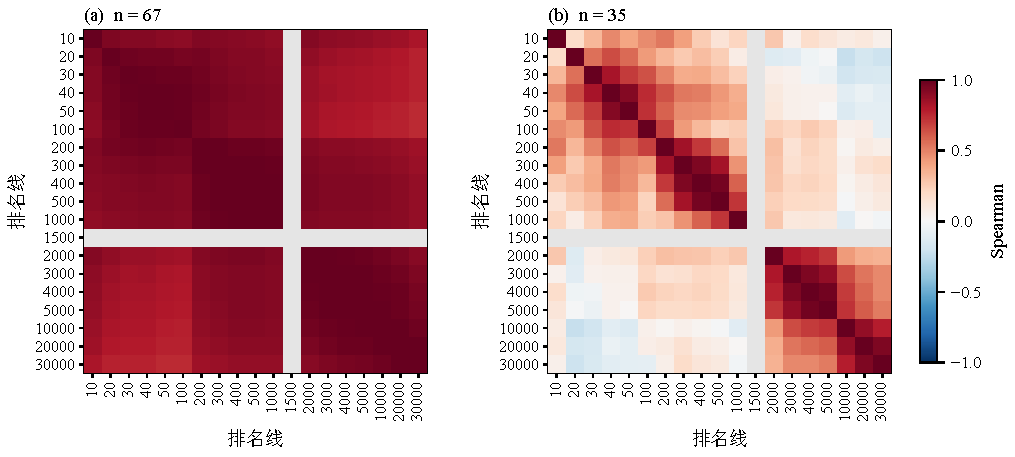
\includegraphics[width=15.8cm,height=\textheight,keepaspectratio]{figures/rank_level_and_error_correlations.pdf}
\caption{训练期终分水平与早期因果预测误差的Spearman相关矩阵。左图使用67期训练活动，右图使用35期训练期逐期外推活动。全部19条线保留，灰色T1500行列表示训练期无数据。两图使用相同色标，不把不同样本量的系数差当成一次正式差异检验。}
\label{fig:correlations}
\end{figure}

\subsection{高分数相关不能直接替代残差关系}

表~\ref{tab:correlation}表明，排名区间内终分相关中位数为0.979，跨区间为0.906；调整时间、时长、类型与乐队后仍为0.923和0.735。终分秩变量的第一主成分解释91.2\%的方差，前两个解释97.1\%。这些结果支持存在强共同活动水平，但PCA解释方差不是预测准确率。

\begin{table}[!htbp]
\centering
\caption{训练期不同预测对象的跨线相关}\label{tab:correlation}
\small
\setlength{\tabcolsep}{4pt}
\renewcommand{\arraystretch}{1.18}
\begin{tabularx}{\linewidth}{L r r r}
\toprule
分析对象 & 共同活动数 & 区间内中位相关 & 跨区间中位相关 \\
\midrule
最终分数水平 & 67 & 0.979 & 0.906 \\
条件调整后的终分 & 67 & 0.923 & 0.735 \\
半程之后的剩余增长 & 66 & 0.653 & 0.452 \\
早期同期原始误差 & 35 & 0.699 & 0.197 \\
中期同期原始误差 & 35 & 0.374 & 0.176 \\
末期同期原始误差 & 35 & 0.308 & 0.120 \\
上期到本期早期原始误差 & 34对连续活动 & 0.003 & −0.066 \\
\bottomrule
\end{tabularx}
\par\vspace{4pt}
\begin{minipage}{\linewidth}\footnotesize\setstretch{1.1}
注：四个固定排名区间见第4.3节。不同分析对象的有效共同活动数不同；相关中位数不等于某一个指定线对的系数，也不具有因果含义。
\end{minipage}
\end{table}

T1000/T2000的训练终分相关为0.927，但半程剩余增长相关仅为0.104，早期原始误差相关为0.268，其5活动块区间为{[}−0.109，0.633{]}。相反，T400/T500的早期误差相关为0.961。将所有排名共同压入单一残差因子，会混合这些不同结构。跨期误差的绝对相关中位数仅约0.10至0.13；较保守的循环位移与全局BY筛查没有留下 \(q<0.05\) 的关系，但34对活动所允许的离散显著性水平和多重校正使检验力有限，不能据此证明信号不存在。

\subsection{神经结构扩展与匹配消融}

最新一轮共享输出网络测试为6.716\%，相对独立参考增加0.045个百分点，活动配对区间{[}−0.200，0.268{]}跨零。增加每线专属头后为7.240\%；相对共享输出增加0.524个百分点，区间为{[}0.261，0.844{]}。专属头在当前样本规模下未形成预期收益。相关线分支相对专属头改善0.027个百分点，但区间{[}−0.081，0.031{]}跨零；进一步加入阶段图与注意力增加0.005个百分点，区间同样跨零。

\begin{table}[!htbp]
\centering
\caption{神经结构的逐层匹配消融}\label{tab:ablation}
\small
\setlength{\tabcolsep}{4pt}
\renewcommand{\arraystretch}{1.18}
\begin{tabularx}{\linewidth}{L C{1.65cm} C{3.25cm} C{3.25cm}}
\toprule
比较 新方法减对照 & \shortstack{差值 /\\百分点} & 活动配对95\%区间 & 5活动块95\%区间 \\
\midrule
共享输出减独立参考 & +0.045 & [−0.200，0.268] & [−0.159，0.238] \\
专属头减共享输出 & +0.524 & [0.261，0.844] & [0.214，0.871] \\
相关线减专属头 & −0.027 & [−0.081，0.031] & [−0.074，0.028] \\
阶段注意力减静态相关线 & +0.005 & [−0.052，0.065] & [−0.042，0.053] \\
\bottomrule
\end{tabularx}
\end{table}

此前多线门控网络相对相同四专家固定组合改善0.055个百分点，配对区间为{[}−0.089，−0.021{]}；但其相对独立暖校正仅改善0.013个百分点，区间{[}−0.074，0.045{]}跨零。这说明``优于固定组合''与``优于最简单匹配参考''不是同一结论。上一轮验证选择的图校正测试为6.938\%，相对独立参考增加0.267个百分点，配对区间{[}0.100，0.426{]}。图~\ref{fig:correlations}中的相关结构并未自动转化为稳定预测收益。

\begin{figure}[!htbp]
\centering
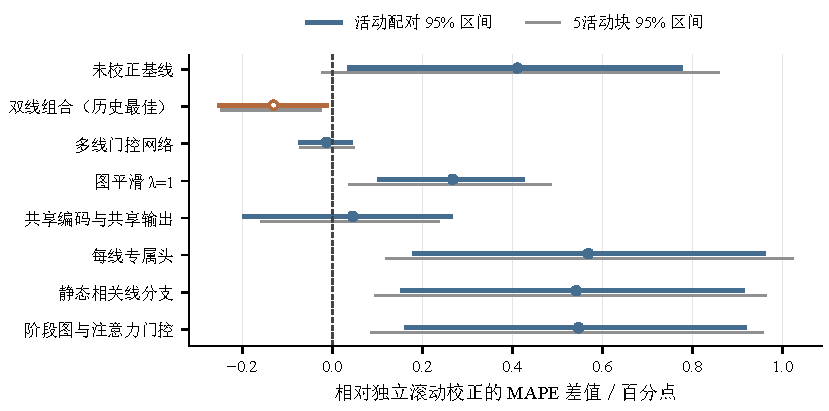
\includegraphics[width=15.8cm,height=\textheight,keepaspectratio]{figures/matched_model_error_differences.pdf}
\caption{相同19线测试面板上的模型差值与不确定性。负值表示优于独立暖校正，粗线为活动配对区间，细灰线为5活动循环块区间。空心点标识历史探索后关注的双线组合。所有区间均未进行多方法选择校正。}
\label{fig:differences}
\end{figure}

\subsection{时间节点与排名异质性}

双线组合在25\%、50\%、75\%、90\%和95\%进度的19线MAPE依次为10.403\%、7.962\%、5.858\%、3.844\%和2.927\%。结束前24、6和1小时相应为3.918\%、2.283\%和1.404\%。总体误差随信息积累而下降，但并非严格单调；结束前0.5与0.25小时约为1.440\%，可能受到覆盖差异和终点修订等因素影响，不能仅凭汇总曲线识别其机制。

开始后1小时没有合格案例，不能报告为零误差；开始后3小时仅8期、8个前缀，MAPE为31.328\%。早期与末期的案例覆盖不同，图~\ref{fig:origins}为冻结可用面板上的描述，不能解释成同一批活动在所有时点上的配对改善。完整时点与共同面板信息随补充数据提供。

\begin{figure}[!htbp]
\centering
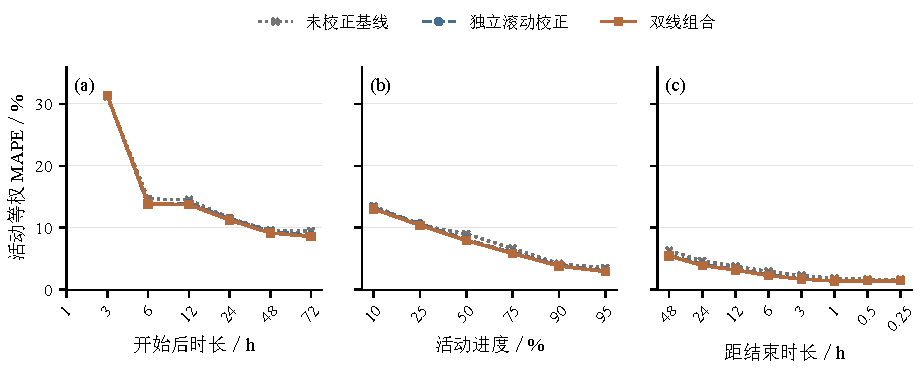
\includegraphics[width=15.8cm,height=\textheight,keepaspectratio]{figures/error_by_forecast_origin.pdf}
\caption{三个时间轴上的19线MAPE。各曲线使用相同方法间案例，但不同时间点的可用活动覆盖可能不同。开始后1小时为空缺，3小时仅有8期。右图横轴由距结束48小时递减至0.25小时。}
\label{fig:origins}
\end{figure}

图~\ref{fig:ranks}与表~\ref{tab:allranks}显示排名异质性。T1000由未校正19.072\%降至独立校正10.797\%，再降至双线组合8.543\%；T2000依次为4.966\%、4.687\%和4.545\%。相对于独立暖参考，双线组合只改变这两条线，其余17档预测完全相同。T10和T20在独立校正后反而高于未校正基线，表明校正并非对每条线都有效；本研究没有按已知测试逐线选择开关。

\begin{table}[!htbp]
\centering
\caption{全部排名线的测试覆盖与MAPE}\label{tab:allranks}
\small
\setlength{\tabcolsep}{4pt}
\renewcommand{\arraystretch}{1.18}
\begin{tabular}{l C{2.2cm} r r r r r}
\toprule
排名 & \shortstack{训练／验证\\曲线数} & 测试活动 & 测试前缀 & 未校正 / \% & 独立校正 / \% & 双线组合 / \% \\
\midrule
T10 & 67／13 & 13 & 248 & 10.880 & 12.127 & 12.127 \\
T20 & 67／14 & 16 & 281 & 10.176 & 10.917 & 10.917 \\
T30 & 67／14 & 16 & 281 & 8.258 & 8.828 & 8.828 \\
T40 & 67／14 & 16 & 281 & 8.357 & 7.906 & 7.906 \\
T50 & 67／14 & 16 & 281 & 8.564 & 8.785 & 8.785 \\
T100 & 67／14 & 16 & 281 & 7.637 & 7.749 & 7.749 \\
T200 & 67／14 & 16 & 281 & 6.549 & 5.906 & 5.906 \\
T300 & 67／14 & 16 & 281 & 5.183 & 5.423 & 5.423 \\
T400 & 67／14 & 16 & 281 & 6.455 & 6.028 & 6.028 \\
T500 & 67／14 & 16 & 281 & 8.785 & 6.812 & 6.812 \\
T1000 & 67／14 & 16 & 281 & 19.072 & 10.797 & 8.543 \\
T1500 & 0／0 & 14 & 242 & 8.402 & 8.444 & 8.444 \\
T2000 & 67／14 & 16 & 279 & 4.966 & 4.687 & 4.545 \\
T3000 & 67／14 & 16 & 279 & 2.998 & 3.229 & 3.229 \\
T4000 & 67／14 & 16 & 279 & 2.816 & 3.181 & 3.181 \\
T5000 & 67／14 & 16 & 279 & 3.409 & 3.479 & 3.479 \\
T10000 & 67／14 & 16 & 277 & 3.360 & 3.316 & 3.316 \\
T20000 & 67／14 & 16 & 267 & 3.574 & 3.729 & 3.729 \\
T30000 & 67／14 & 16 & 260 & 4.941 & 5.336 & 5.336 \\
\bottomrule
\end{tabular}
\end{table}

T1500首次出现时依赖共享排名信息。其活动结束后，后续V3活动允许使用已经到达的真实反馈，因此14期平均不能称作14次始终没有本线历史的零样本预测。早期缺失也意味着该档未参与验证阶段的参数选择。

\begin{figure}[!htbp]
\centering
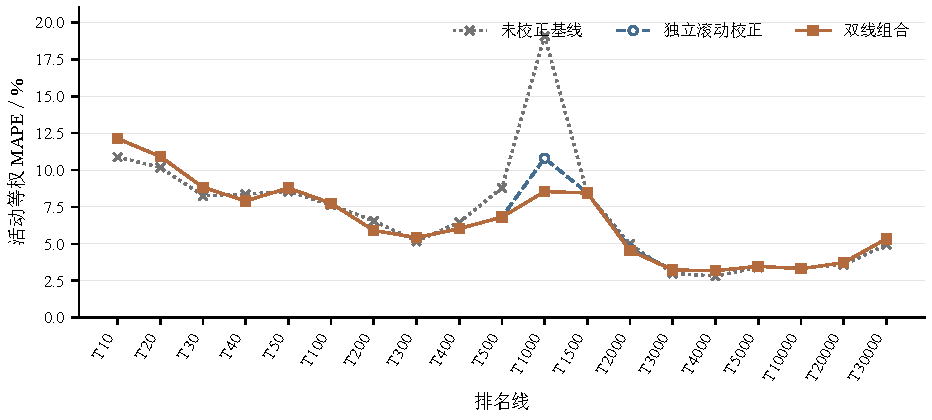
\includegraphics[width=15.8cm,height=\textheight,keepaspectratio]{figures/errors_across_all_ranks.pdf}
\caption{全部19条排名线的测试误差。独立校正与双线组合在其余17档完全重合；整体MAPE的改善集中于T1000及T2000，不能外推为所有档位一致获益。}
\label{fig:ranks}
\end{figure}

\subsection{活动类型与乐队分组}

双线组合在challenge、festival、live\_try、medley、mission\_live和versus六类活动中的MAPE分别为8.690\%、6.848\%、5.808\%、7.220\%、6.712\%和5.285\%，对应活动数为3、1、4、1、3和4。乐队分组中，混合乐队4期的MAPE为7.931\%，Poppin'Party两期为6.034\%，RAISE A SUILEN两期为5.748\%，Morfonica两期为7.526\%。这些分组的活动类型、时间、持续时长与排名覆盖同时变化，不能据此认定乐队身份或规则类型造成了误差差异。

较早的``类型与乐队分组收缩''两线残差实验测试为8.275\%，没有超过同轮冷启动EWMA的7.995\%。仅增加活动条件并不能保证改善；细分后的样本量更小，正则化与跨组共享需要同时考虑。完整类型和乐队表保留在补充材料，主文不据测试分组差异追加参数选择。

\FloatBarrier
\section{讨论}

\subsection{误差状态比网络规模更接近当前证据}

固定留出下较低的训练与验证误差、后续活动较高的测试误差，以及同一滚动基础预测经校正后的改善，共同支持研究近期误差状态的必要性。这些现象与非平稳环境下的偏差变化相容，但尚未单独识别概念漂移、元数据误差、选择偏差和有限样本波动各自的贡献。因此，``所有瓶颈均来自漂移''超出了当前证据。

锚点与差异分解为T1000和T2000提供不同记忆速度，比强制全线共享同一残差更有针对性。T2000的较慢锚点和较快的线间差异项，可以在不引入大量自由参数的情况下表达相对误差变化。其成功也并不依赖T1000/T2000拥有最高的同期残差相关。更合理的解释是该分解在这个面板上适配了异质的偏差状态，而不是发现了两线之间稳定的因果传递。

\subsection{共享何种信息比是否共享更关键}

终分强相关说明活动具有共同水平，却不说明``当前已经解释掉的水平''仍然留在剩余误差中。同期残差在预测时尚未知晓，跨期残差传播还额外要求其关系具有可延续性。表~\ref{tab:correlation}中关系从终分到剩余增长、再到跨期误差逐步减弱，解释了为什么高相关统计本身不能作为共享校正成功的充分证据。

每线专属头增加可辨别参数，但独立监督单位仍然只有几十期活动。不同快照不能替代更多独立活动；专属参数也可能吸收不稳定的组别差异。神经网络未获益与过度灵活、小样本和分布变化等解释相容，本文没有通过实验逐一分离这些机制。另一方面，相关线分支相对专属头存在小幅改善，说明局部迁移并非完全没有潜力；其区间跨零，尚不足以替换简单参考。

\subsection{从回溯实验到持续预测系统}

生产系统与离线评分分开维护：每15分钟同步公开分数，依据合法已结束历史准备基础模型；活动开始时固定模型及校正状态，持续输出当前前缀预测；活动结束且通过终点质量检查后，已发布原始预测的误差才回灌后续活动。实时反馈优先于回溯初始化记录，替换旧种子时保留历史；训练失败时保留已有可用版本。这里的``自动训练''是按固定配方重估模型与更新误差状态，不是根据已知测试成绩自动搜索并换算法。

截至2026年11月18日，本地验收包含391项测试，校正层对65期、21117条封存预测的回放最大绝对差为 \(2.98\times10^{-8}\) EP，属于浮点舍入量级。实际后台联网周期已更新19档数据。这些检查验证软件运行、版本一致性和信息守卫，不构成新的预测精度评估。生产已将双线组合设为新活动默认；正在进行的活动329保留期初原校正快照，不把历史最佳配方说成已在本期接受了前瞻验证。

\subsection{局限与后续验证}

首先，只有16期测试活动，且队列在早期研究中已经暴露；验证组也被多轮使用。事前登记某一次后续菜单可以约束该轮操作，但不能使被探索过的队列重新成为全新盲测。其次，活动、角色与卡牌元数据来自回溯快照，虽按国服发布时间过滤卡牌并严格控制终分到达时间，仍缺少全部历史时点元数据存档，无法完全重建当时可得信息。

再次，结果来自同一游戏、同一服务器和选定密集时期，无法直接推广到不同游戏机制或采样系统。缺失前缀若与活动条件有关，可用面板本身也可能存在选择偏差；T1500和T10尤其需要单独报告。活动时间间隔不等、误差可能存在趋势，均会削弱块重采样和循环位移方法的近似假设。模型比较的边际区间未校正多重探索，结论应保持探索性。

最后，当前输出为点预测。总体MAPE较低不代表某一期、某一排名或早期预测可靠，RMSE也未随百分比误差同步改善。后续应将当前组合、独立暖校正和少量预先固定候选，在未参与任何分析的新活动上封存影子预测；待终分到达后按相同排名与时间点评分，并同时检查尾部误差及区间覆盖。新增样本量应按活动数量和目标效应大小规划，而不是任意把更多快照算作独立样本。本文不从既有测试继续选择下一组参数。

\section{结论}

本文针对音乐游戏活动排名终分预测，建立了共享活动归属的固定留出、时间网格和逐活动滚动评测体系，并以2024年1月29日起97期密集采样活动为研究队列。在相同19线V3面板上，独立暖启动误差校正将活动等权MAPE由7.082\%降至6.671\%；历史双线组合达到6.540\%，改善主要集中于T1000。四种新增共享编码与相关线神经结构未在事前验证选择中替代简单参考。

统计结果表明，强共同分数水平、同期剩余误差和跨期可预测误差属于不同层次的关系。对于当前独立活动数有限的数据，优先约束信息时间边界、区分排名异质性并进行收缩校正，比依据水平相关直接扩大共享网络更符合现有证据。双线组合已作为后续活动的生产默认配方，但其精度优势仍需未参与探索的新活动前瞻验证。

\FloatBarrier
\section*{数据与代码可用性}

公开数据来源为Bestdori活动与排名接口\citep{bestdori2026data}，研究代码仓库入口为\href{https://github.com/AhsokaTano26/BanG-DreamActivity-fraction-prediction/tree/research/innovation-20261113}{AhsokaTano26 BanG Dream Activity fraction prediction}。本文随稿提供329组历史结果汇总、19线匹配比较、按排名及时间点的明细、相关矩阵、图表源数据和生成脚本。精确研究版本以随稿来源清单中的SHA-256、冻结数据指纹和各运行身份为准；公共仓库分支与本地未发布工件的版本状态分别记录于交付说明。

新V1、V2两线、V2的19线、V3两线及V3的19线数据指纹前12位分别为80e354c3a534、d057beca6597、8ffd781fc9f4、85f5924e0b90及db4e9b9c84bd；完整指纹随补充数据提供。论文图表从既有封存结果提取，不新增模型训练，不改变冻结分组、线上参数或原始预测。


\bibliographystyle{unsrtnat}
\bibliography{references}
\end{document}
